\documentclass[10pt,letterpaper]{article}
\usepackage[margin=1in]{geometry}
\usepackage{graphicx}
\usepackage{enumitem}
\setlist{nosep}
\setlength{\parindent}{0pt}
\setlength{\parskip}{0.5em}
\usepackage[font=small,skip=2pt]{caption}
\usepackage{float}
\usepackage[hidelinks]{hyperref}

\title{Lab 2 - Linguistics Data, Stat 215A, Fall 2026\vspace{-2em}}
\date{}

\begin{document}
\maketitle

\section{Introduction}\label{introduction}

Dialectology is the study of how language varies, especially across geography, and dialectometry is the quantitative measurement of those differences \cite{nk2003}. Early dialectologists found that variation is complex and cannot be reduced to simple descriptions, which created a need for computational techniques that can handle large amounts of data \cite{nk2003}. A central question is whether language variation is organized into distinct dialect areas, each separated from its neighbors, or whether it is better described as a continuum or ``chain'' of dialects that change gradually from place to place \cite{nk2003}. A second difficulty is that any single word or pronunciation is only weakly tied to geography: for almost every feature that seems to define a region, there are exceptional places inside and outside it. Séguy's observation, which started dialectometry, is that an aggregate of many features can show geographic structure more reliably than any one feature \cite{nk2006}.

This report applies that idea to the Vaux dialect survey \cite{vaux}, in which 47{,}471 respondents across the United States chose among answers to multiple-choice questions about words they use, together with where they live. I use the 67 word-choice questions together to ask the following:
\begin{itemize}
\item Do people form groups with similar answers, and do these groups relate to geography?
\item Are the groups separate, or do they blend into each other in a continuum, and from where to where?
\item Which questions most separate the groups?
\item How reliable are the groups when the data or the algorithm is perturbed?
\end{itemize}

The rest of the report is organized as follows. Section~\ref{data} describes the data and the cleaning steps, and compares two pairs of questions using maps and measures of association. Section~\ref{dimension-reduction} encodes the answers as binary variables and uses PCA and t-SNE to look for structure. Section~\ref{clustering} clusters respondents with k-means and a Gaussian mixture model and checks whether the clusters follow geography. Section~\ref{stability} tests how stable the clusters are to different starting points and resampling of the data, and Section~\ref{conclusion} discusses what the results do and do not show.

\section{The Data}\label{data}

The data come from an online survey of American English dialects. Each of $n = 47{,}471$ respondents answered up to 67 multiple-choice questions about everyday words and pronunciations (Q050--Q121; 468 answer options in total) and gave their city, state and ZIP code, from which a latitude and longitude are recorded. Answers are stored as integer codes for the listed options, so the codes are labels, not quantities.

\paragraph{Link to the domain problem.} We want to know how dialect varies across the US: which words are used where, and whether the differences form distinct regions or a smooth gradient. Each respondent gives a vector of 67 categorical choices and a place, so we can ask whether people who answer alike also live near each other. Two limitations are that respondents are self-selected online volunteers, and that the location is where they live, not necessarily where they grew up.

\subsection{Data Cleaning}\label{data-cleaning}

All steps are done in order in one notebook, and every removed row is counted (Table~\ref{tab:cleaning}).

\begin{enumerate}
\item \textbf{Zeros mean ``no response.''} Of the answers, 100{,}902 (3.2\%) are coded 0, which is not an answer option, so these were recoded to missing (NaN). They occur only for respondents with ID $\le 16{,}970$ (Figure~\ref{fig:missingness}, left), perhaps because the survey later required an answer.
\item \textbf{Respondents who skipped most questions.} Most skip a few, but a second group skips nearly all (Figure~\ref{fig:missingness}, right); 1{,}040 answered none. I removed respondents who skipped more than half of the questions (1{,}287). The cutoff is a judgment call, but the result is insensitive to it: any cutoff from 20 to 60 skipped questions removes between about 1{,}100 and 1{,}400 respondents. Respondents with only a few skips are kept, with those answers left missing.
\item \textbf{Missing location.} 991 of the remaining respondents have no latitude/longitude and cannot be placed on a map, so they were removed.
\item \textbf{Alaska and Hawaii.} These points (Figure~\ref{fig:allpoints}) are isolated and would stretch every map, so only longitude $-125$ to $-66$ and latitude 24 to 50 were kept (198 removed). Conclusions apply to the lower 48 states.
\item \textbf{Flagged, not removed.} The state field is free text, and 159 raw rows contain an invalid state code (e.g.\ ``XX''). Additionally, 142 respondents have coordinates over $15^\circ$ from their typed state. Since latitude/longitude is used rather than the typed state, these rows were kept and given indicator columns. ZIP codes were read as text so that leading zeros are kept.
\end{enumerate}

The cleaned data have 44{,}995 respondents (94.8\% of the raw data), all with coordinates in the contiguous US and at least half of the questions answered.

\begin{table}[h]
\centering
\small
\begin{tabular}{lrrr}
\hline
Step & Removed & Remaining & \% of raw kept \\
\hline
Raw data (0 recoded to missing) & 0 & 47,471 & 100.0 \\
Skipped more than half the questions & 1,287 & 46,184 & 97.3 \\
Missing latitude/longitude & 991 & 45,193 & 95.2 \\
Outside the contiguous US & 198 & 44,995 & 94.8 \\
\hline
\end{tabular}
\caption{Respondents removed at each step, applied in this order.}
\label{tab:cleaning}
\end{table}

\begin{figure}[h]
\centering
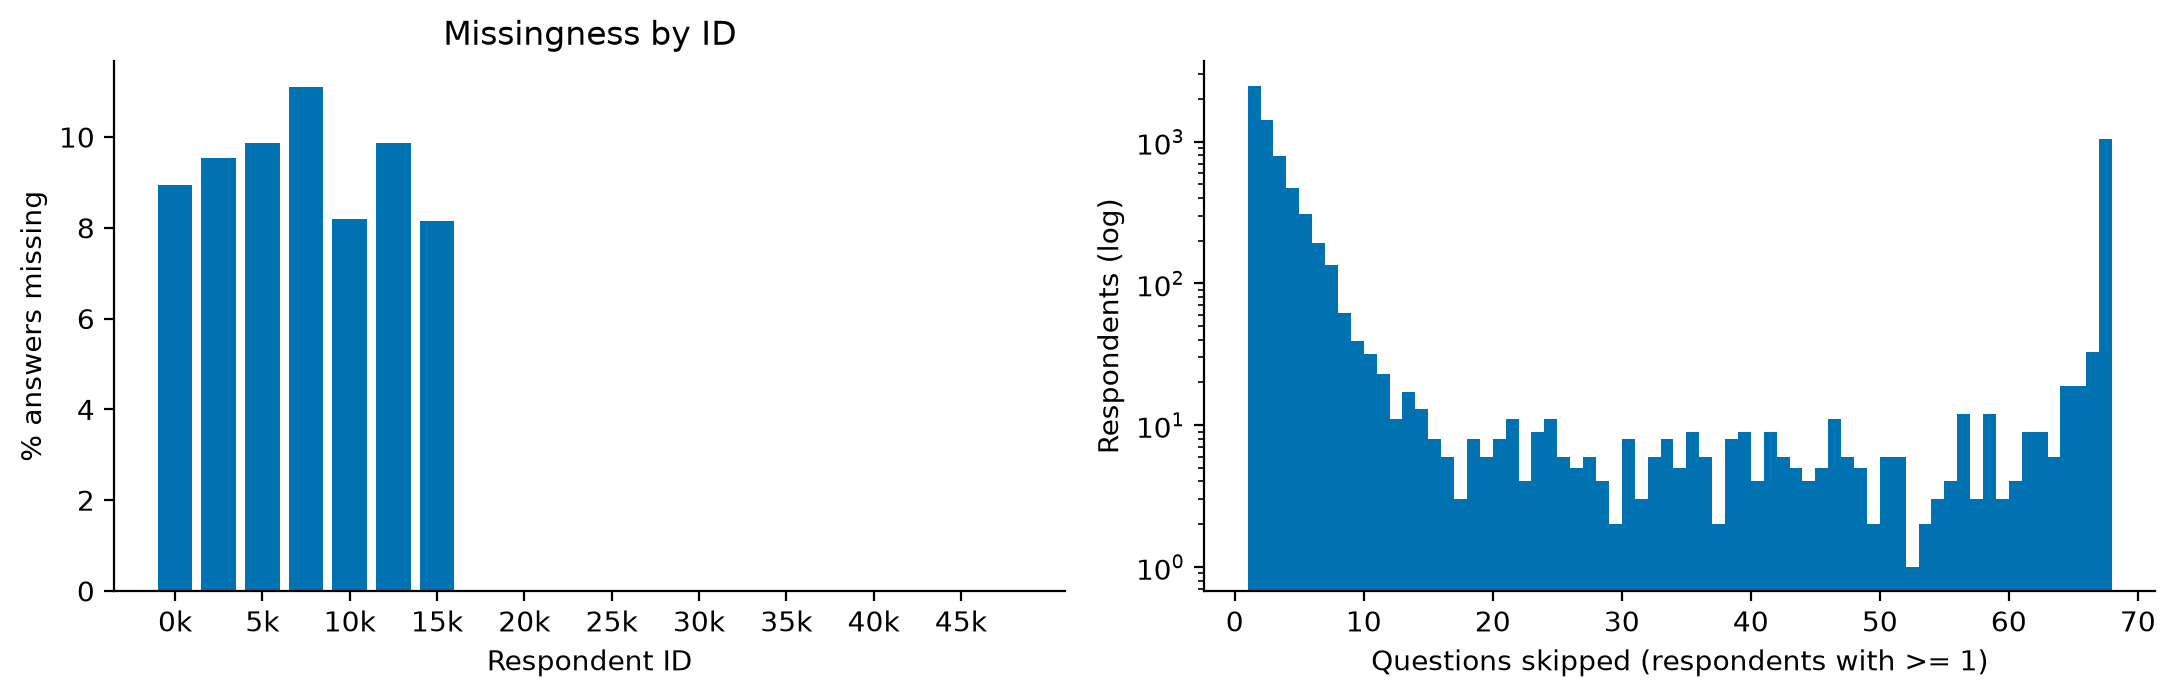
\includegraphics[width=0.85\textwidth]{figures/clean_missingness.png}
\caption{Left: percent of answers missing by respondent ID (bins of 2{,}500). Right: number of questions skipped among respondents who skipped at least one (log scale).}
\label{fig:missingness}
\end{figure}

\begin{figure}[h]
\centering
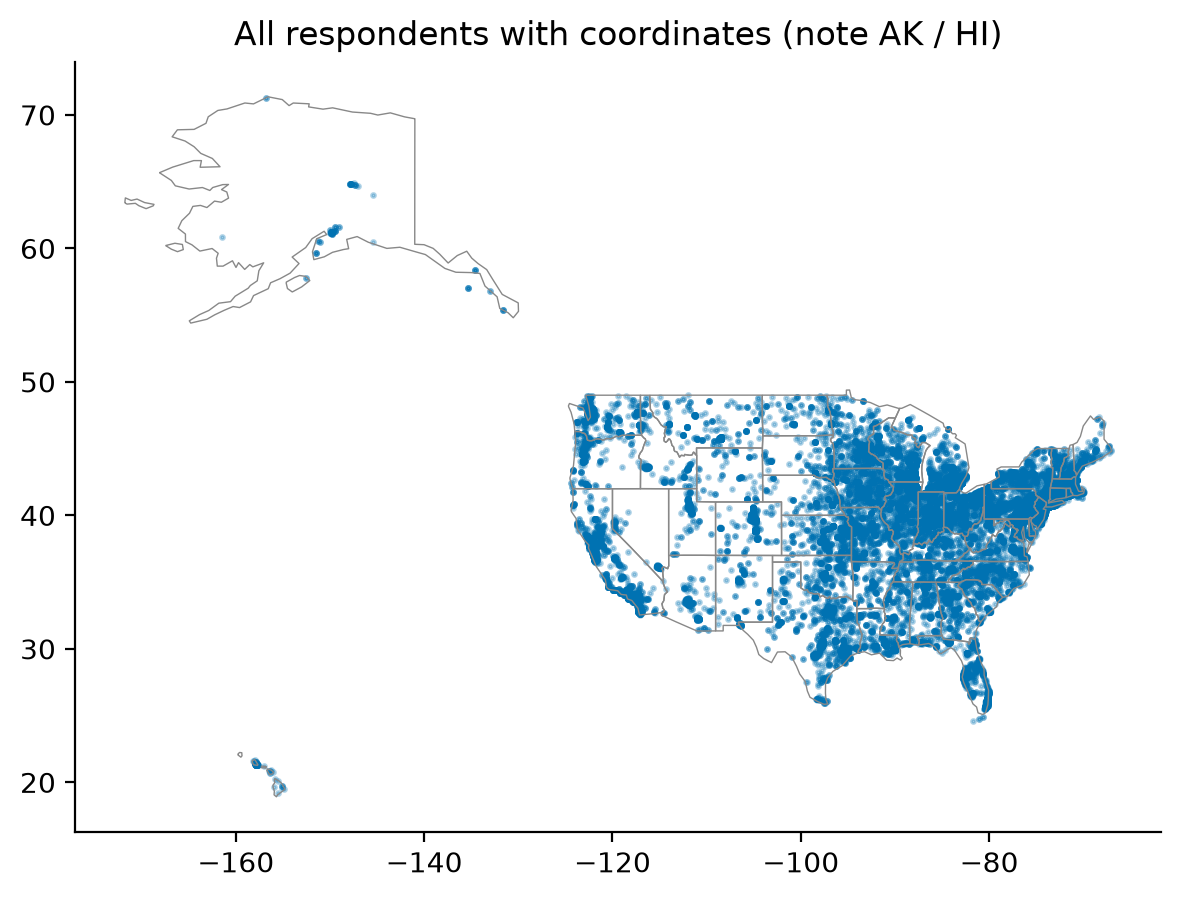
\includegraphics[width=0.5\textwidth]{figures/clean_all_points_map.png}
\caption{All respondents with coordinates, before filtering. Points outside the main map are in Alaska and Hawaii.}
\label{fig:allpoints}
\end{figure}

\subsection{Exploratory Data Analysis}\label{data-exploration}

Two pairs of questions were compared to see how answers relate to each other and to location. The first pair, Q069 and Q071 (what the respondent calls their paternal grandmother and grandfather), are about the same topic, so their answers are expected to be related whether or not geography matters. The second pair, Q066 (the small freshwater crustacean) and Q065 (the glowing summer insect), are unrelated topics that are both known regional markers, so any relationship between them would have to come mostly through geography.

\paragraph{Maps.} Figures~\ref{fig:maps_grand} and~\ref{fig:maps_bugs} show the most common answer to each question in every $1^\circ \times 1^\circ$ latitude--longitude cell. Cells with fewer than 5 respondents are left blank, which is why the West is sparser, and the three most common answers are colored (all others are grey). Each square is a map cell, not a person, and the maps show only the most common answer, not how large its share is.

\begin{figure}[h]
\centering
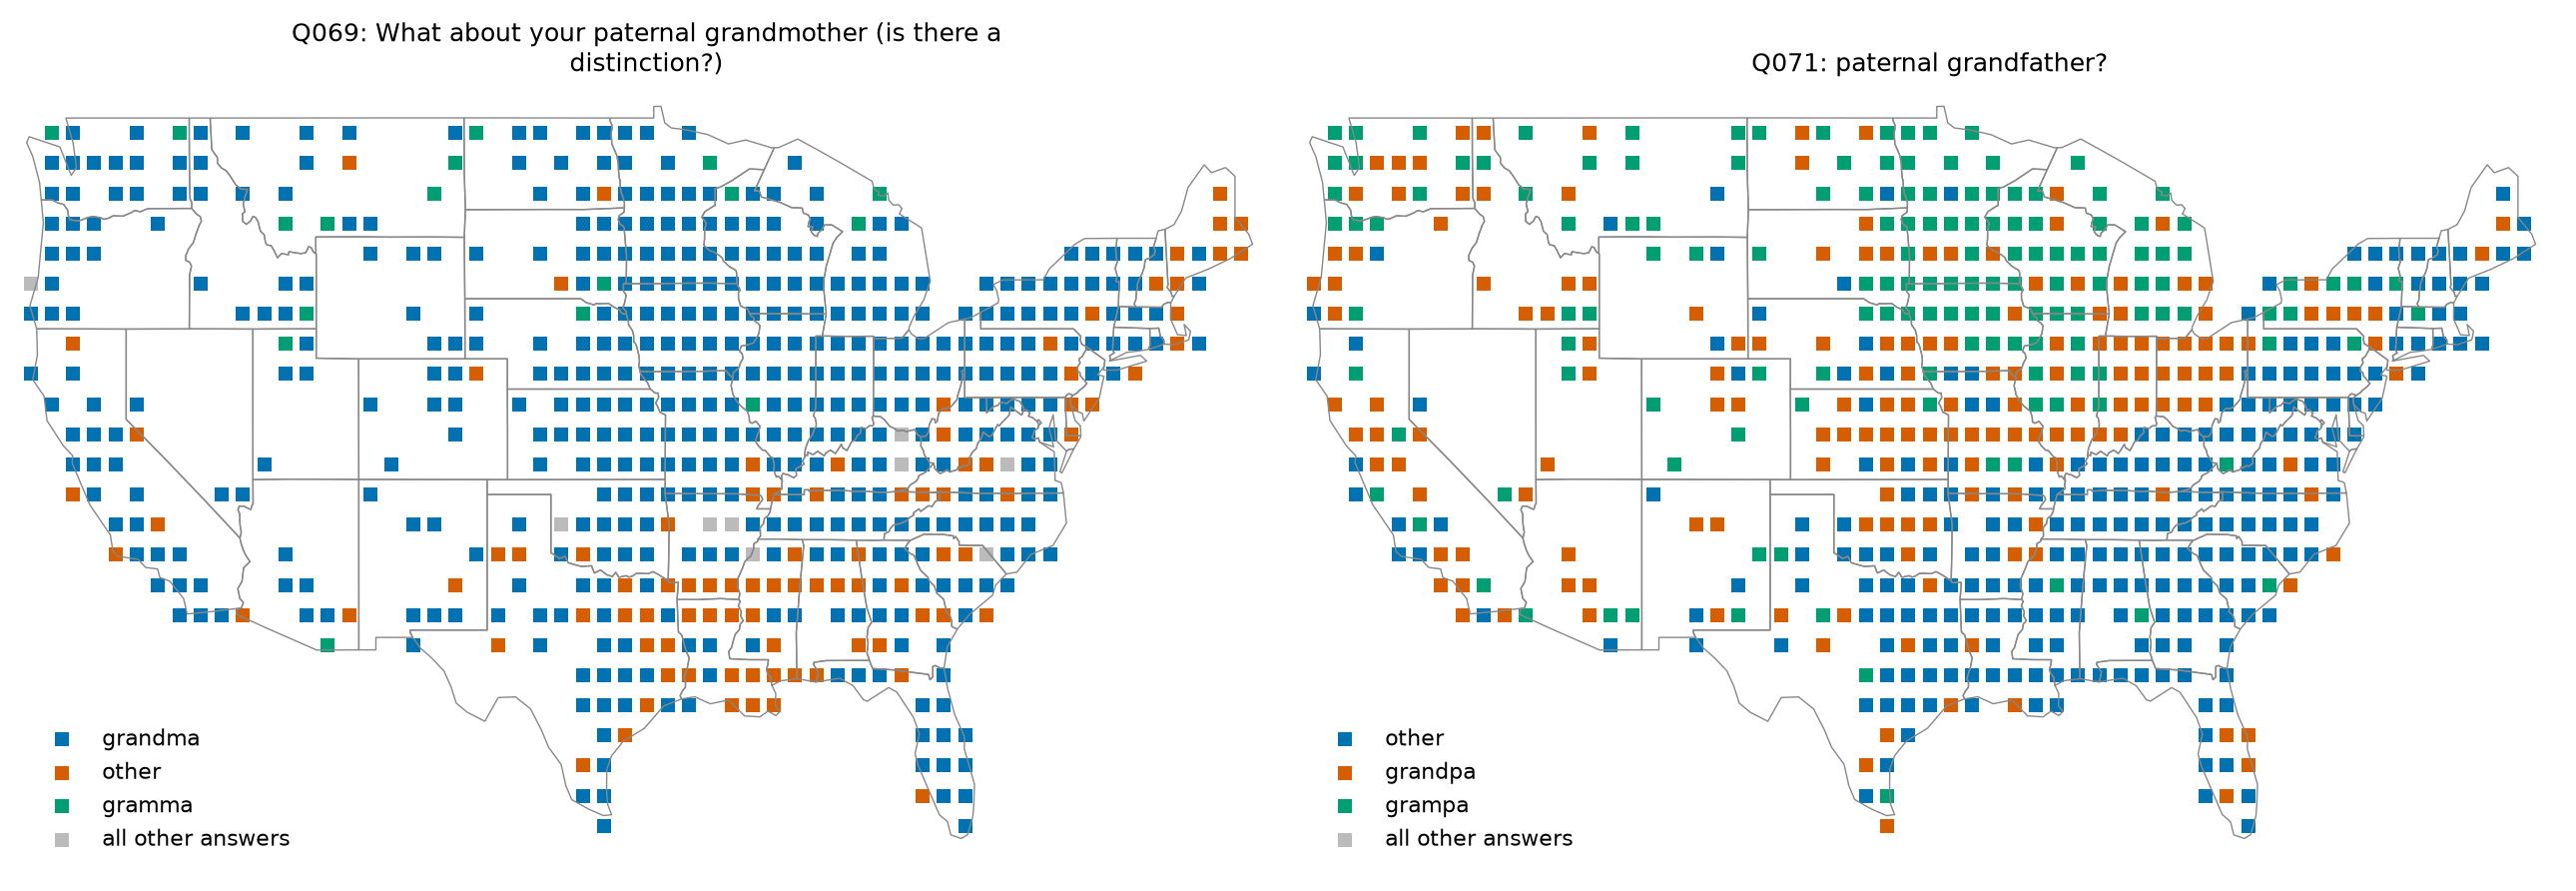
\includegraphics[width=\textwidth]{figures/maps_Q069_Q071.png}
\caption{Most common answer per $1^\circ \times 1^\circ$ cell for Q069 (paternal grandmother) and Q071 (paternal grandfather).}
\label{fig:maps_grand}
\end{figure}

\begin{figure}[h]
\centering
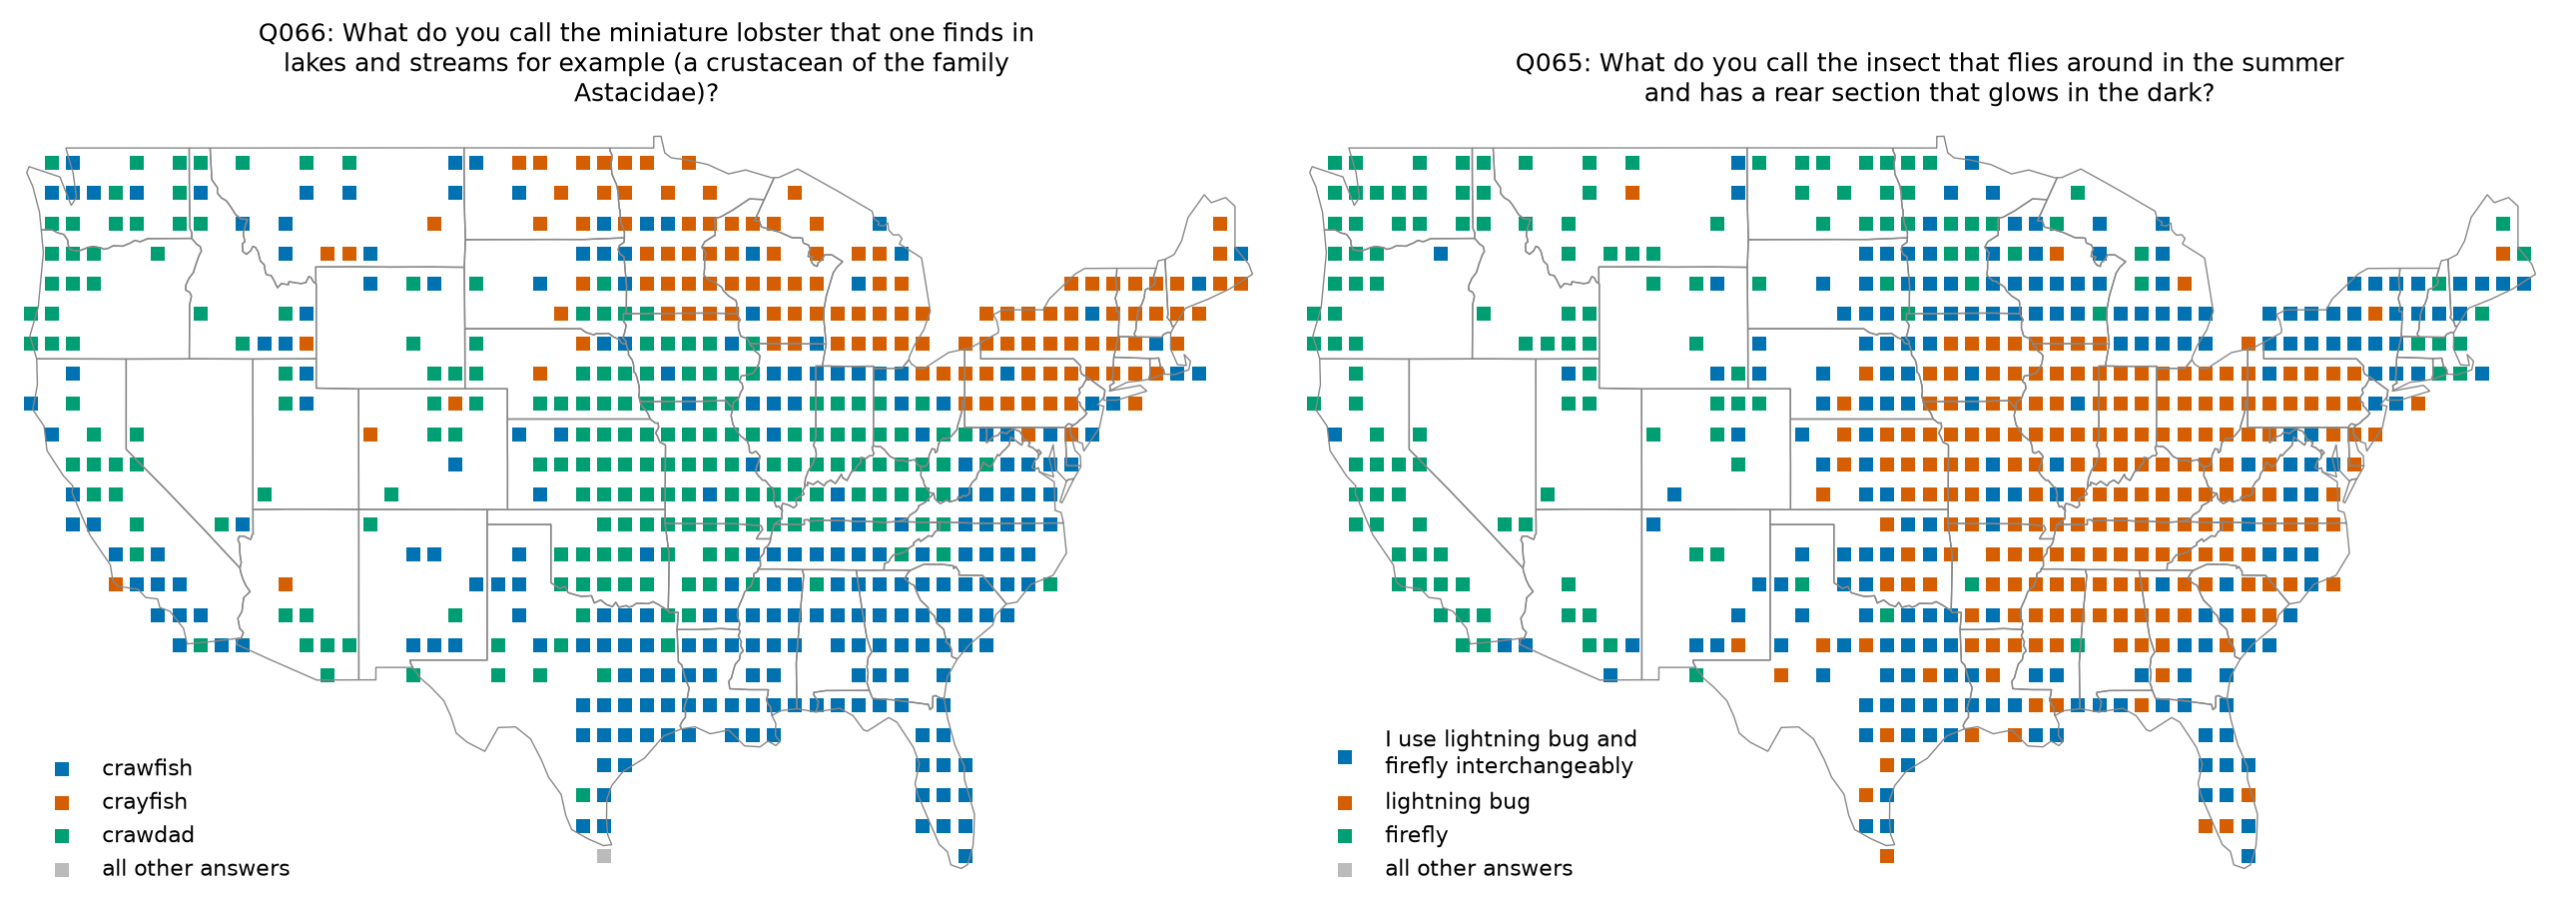
\includegraphics[width=\textwidth]{figures/maps_Q066_Q065.png}
\caption{Most common answer per $1^\circ \times 1^\circ$ cell for Q066 (freshwater crustacean) and Q065 (glowing insect).}
\label{fig:maps_bugs}
\end{figure}

For Q069, ``grandma'' is the most common answer in most cells, and Q071 is much more regional: ``grampa'' is common in the upper Midwest and Pacific Northwest, ``grandpa'' in a band through the central Midwest, and ``other'' (a catch-all category) in the South and Northeast. For the second pair, both questions show clear regional patterns that do not line up. ``Crawfish'' dominates the South, ``crayfish'' the Northeast and Great Lakes, and ``crawdad'' the West and parts of the Midwest, while ``lightning bug'' covers a broad central and eastern area and ``firefly'' the West and far north. Using both words interchangeably is common in the Northeast and along the Gulf coast.

\paragraph{Relationship between the pairs.} For each pair the answers were cross-tabulated using each question's four most common answers (40{,}006 respondents for the first pair and 42{,}731 for the second, about 92\% and 95\% of respondents who answered both). Two measures are reported: Cram\'er's $V$, which is 0 if the questions are independent and 1 if one answer determines the other, and the Goodman--Kruskal $\lambda$, the fraction by which knowing the first answer reduces the errors made when guessing the second answer, compared with always guessing the most common answer. The chi-square test has $p < 10^{-100}$ for both pairs, which is expected with this many respondents, so the size of the association is interpreted rather than the $p$-value.

The grandparent questions are strongly related ($V = 0.42$, $\lambda = 0.46$): Table~\ref{tab:cond} shows that the terms are paired, for example 80\% of ``gramma'' users say ``grampa''. This is likely partly a household naming habit rather than a geographic effect. The crustacean and insect questions are only weakly related ($V = 0.10$, $\lambda = 0.05$), consistent with the two maps showing different regional boundaries. This shows that two questions can each follow geography without being strongly related to each other.

\begin{table}[h]
\centering
\small
\begin{tabular}{lrrrr}
\hline
 & \multicolumn{4}{c}{Q071 (paternal grandfather)} \\
Q069 (paternal grandmother) & grampa & gramps & grandpa & other \\
\hline
gramma & 0.80 & 0.00 & 0.08 & 0.12 \\
grandma & 0.27 & 0.01 & 0.56 & 0.16 \\
grandmother & 0.09 & 0.01 & 0.33 & 0.57 \\
other & 0.10 & 0.01 & 0.12 & 0.77 \\
\hline
\end{tabular}
\caption{Proportion of each Q069 answer (row) that gave each Q071 answer (columns); rows sum to 1.}
\label{tab:cond}
\end{table}

\paragraph{Interactive maps.} The same maps are available as interactive plots (\texttt{map\_Q065.html}, \texttt{map\_Q066.html}, \texttt{map\_Q069.html} and \texttt{map\_Q071.html} in \texttt{report/figures}, opened in a browser with \texttt{plotly.min.js} in the same folder), where hovering over a cell shows its number of respondents and answer shares.

\section{Dimension Reduction}\label{dimension-reduction}

The answer codes are labels (``2'' is not ``twice'' ``1'', and the order of the options is arbitrary), so means, variances and distances between codes are meaningless and the codes cannot be used directly in PCA. Each question was therefore one-hot encoded into one 0/1 column per answer option, giving $p = 468$ columns, and a skipped question has a 0 in every column of its block. PCA and t-SNE were applied to this 44{,}995 $\times$ 468 matrix.

\subsection{PCA: centering and scaling}

PCA was run in two ways. With centering only, the mean of each column is subtracted, so a common answer (high variance, such as a 50/50 split) has more influence than a rare one. With centering and scaling, each column is also divided by its standard deviation, so every answer option has equal influence. Centering only was chosen for two reasons. First, scaling gives a very rare answer the same weight as a very common one, and 39 of the 468 options were chosen by fewer than 0.1\% of respondents. The scaled PCA is visibly affected by this: in the PC3--PC4 plot (Figure~\ref{fig:pca_scatter}, bottom right) a handful of respondents are pulled far from everyone else (down to $-50$), a sign that a few rare answers are driving a component. Second, the question of interest is where large groups of people differ, and the common answers carry that information.

Figure~\ref{fig:pca_scree} shows the variance explained by each component. Under both versions the variance is spread over many components with no clear elbow: for centering only, PC1--PC4 explain 4.1\%, 3.5\%, 2.9\% and 2.1\% of the variance, and the first 20 components together explain only 33\% (17\% with scaling). A respondent's answers are therefore not well summarized by one or two numbers; individual answers vary a lot from person to person, and the regional signal is a small part of that.

\begin{figure}[h]
\centering
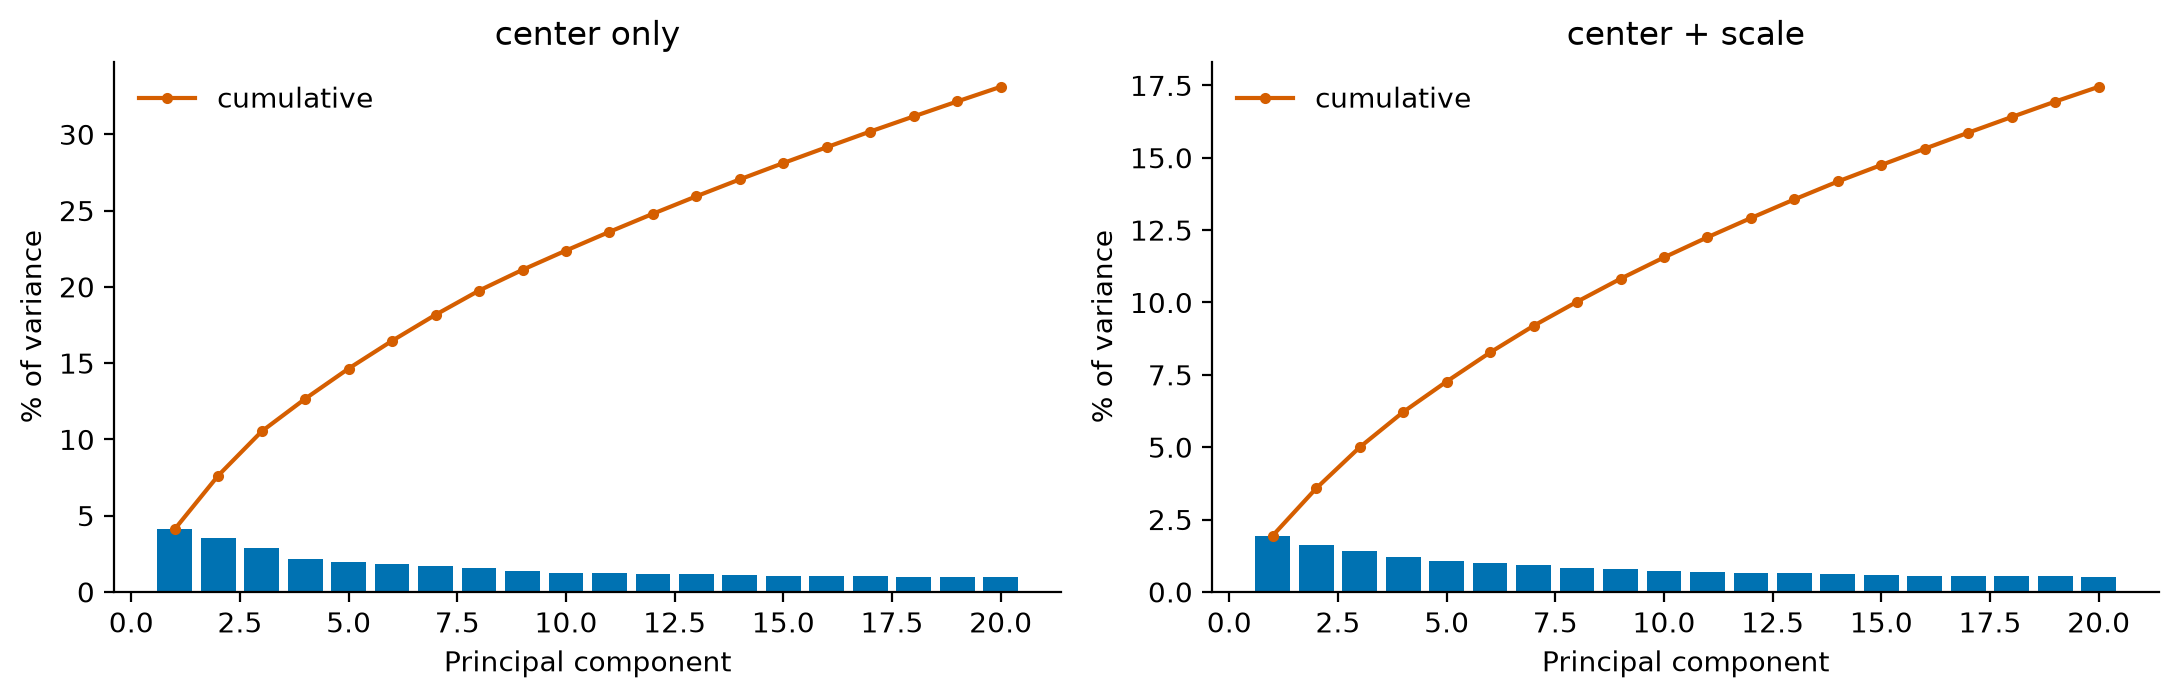
\includegraphics[width=0.9\textwidth]{figures/pca_scree.png}
\caption{Percent of variance explained by each of the first 20 principal components (bars) and cumulatively (line), with centering only (left) and centering plus scaling (right).}
\label{fig:pca_scree}
\end{figure}

\subsection{What the components show}

Even though each component explains little variance, the first two are clearly geographic. Figure~\ref{fig:pca_scatter} plots each respondent by their PC scores, colored by longitude. With centering only, respondents from the east (light) separate from those in the west (dark) along PC1 with no sharp break, and PC3 and PC4 show no clear pattern with longitude. The largest loadings on PC1 are ``sneakers'' versus ``tennis shoes'' (Q073, loadings $+0.27$ and $-0.24$), ``soda'' versus ``pop'' (Q105) and ``sunshower'' (Q080). The largest loadings on PC2 are ``kitty-corner'' versus ``catty-corner'' (Q076), ``drinking fountain'' versus ``water fountain'' (Q103) and ``y'all'' (Q050).

Figure~\ref{fig:pca_maps} shows the mean PC1 and PC2 score in each $1^\circ \times 1^\circ$ cell. PC1 is high in the Northeast and mid-Atlantic and low elsewhere (correlation with longitude 0.42), and PC2 separates the South (low) from the North and West (high; correlation with latitude 0.40). Both vary smoothly across the map, so the components are picking up regional dialect rather than noise, and the two main axes are roughly ``Northeast versus the rest'' and ``South versus the rest''.

\begin{figure}[h]
\centering
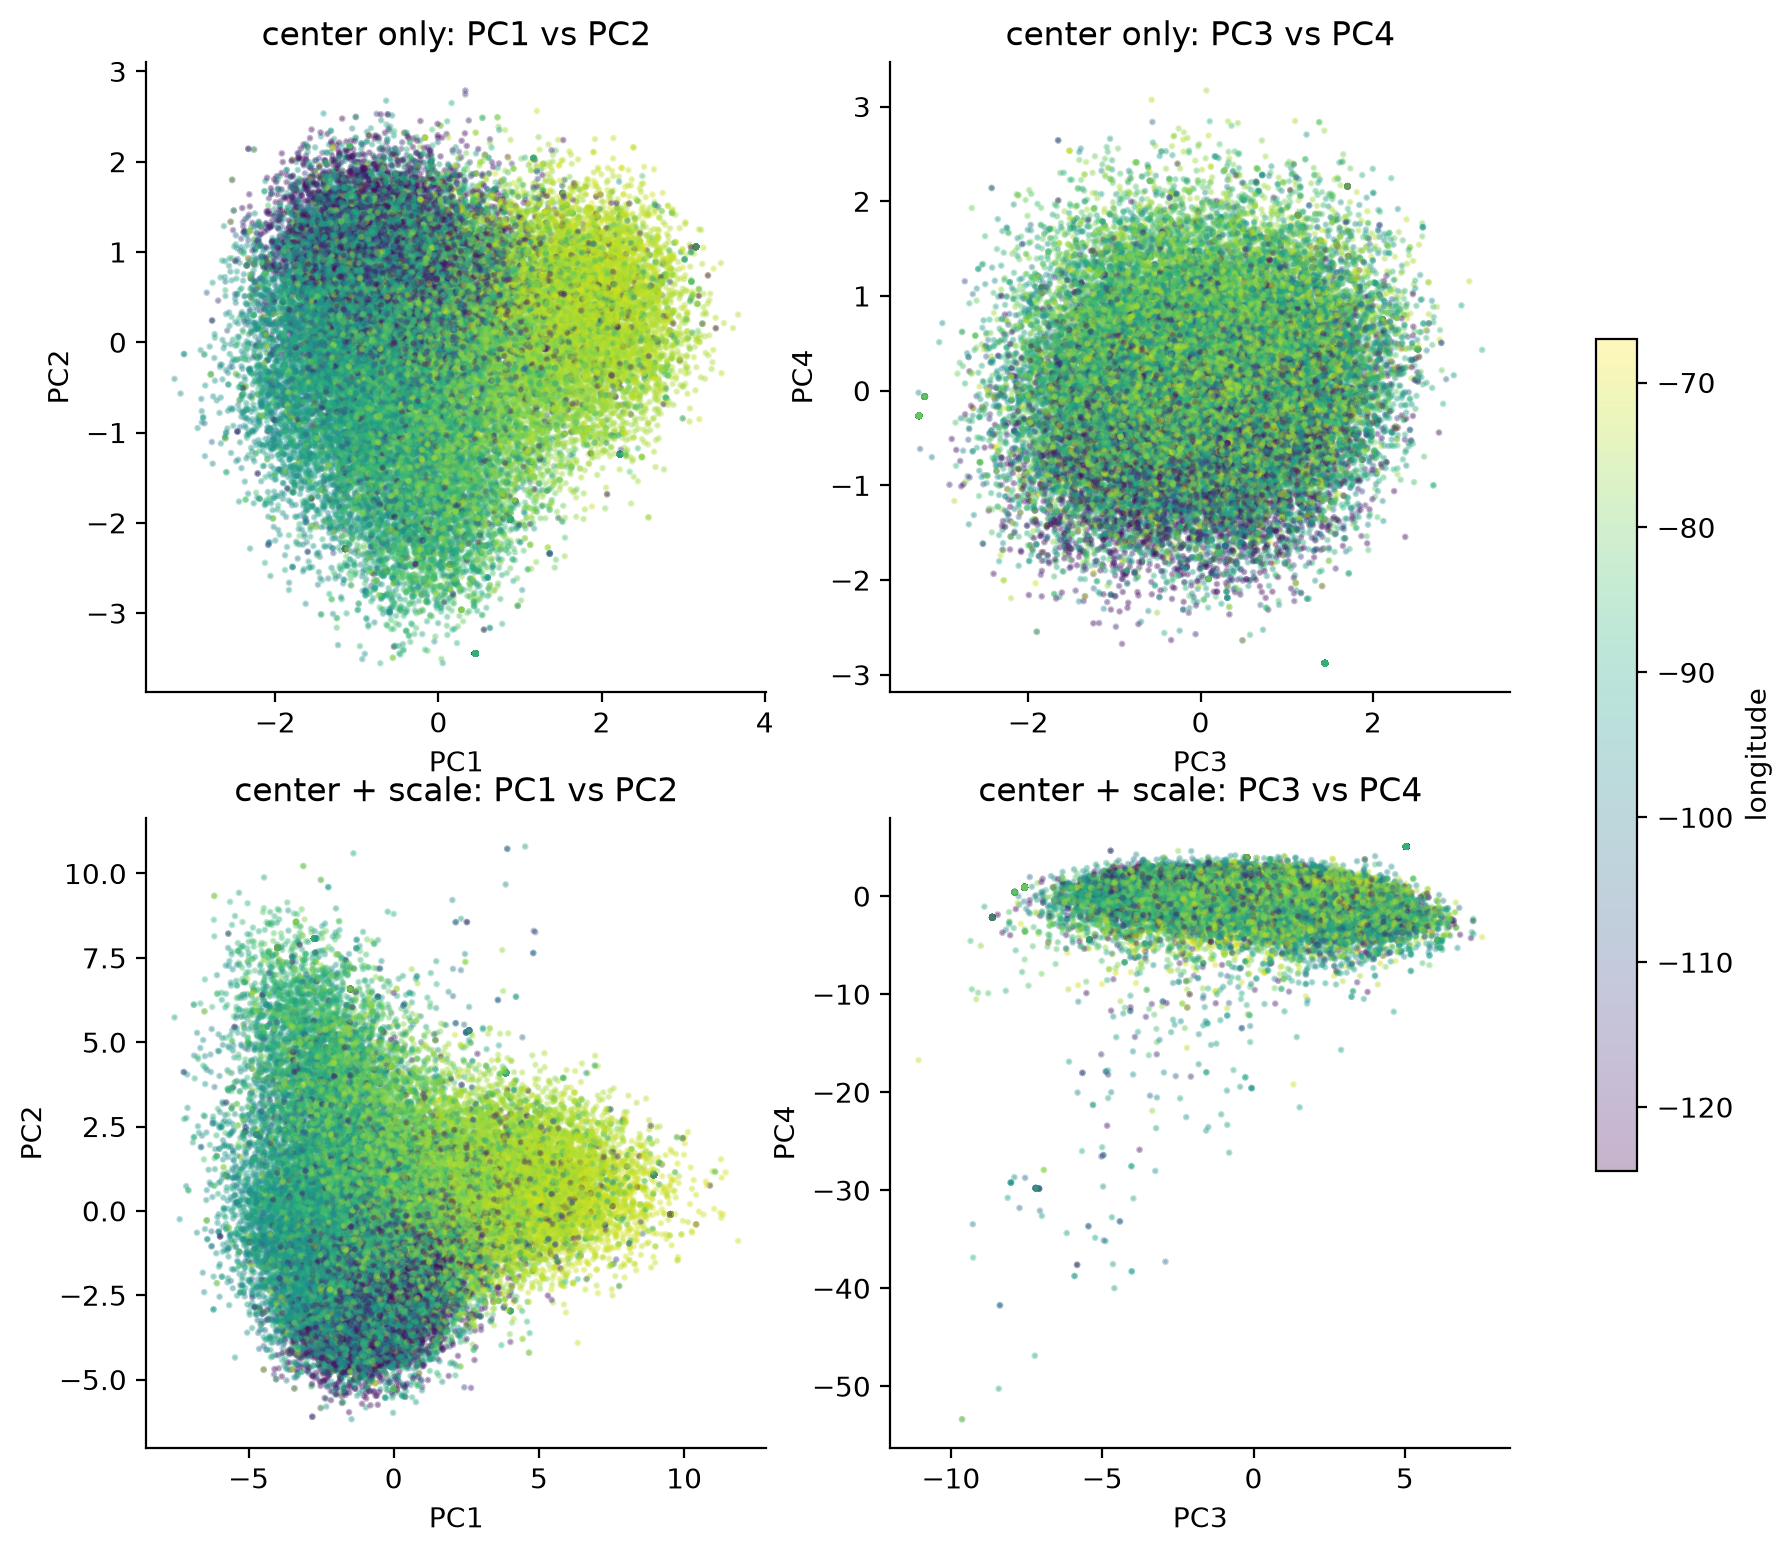
\includegraphics[width=0.62\textwidth]{figures/pca_scatter.png}
\caption{Respondents plotted by PC1 versus PC2 (left) and PC3 versus PC4 (right), for centering only (top) and centering plus scaling (bottom). Color is longitude (dark = west, light = east).}
\label{fig:pca_scatter}
\end{figure}

\begin{figure}[h]
\centering
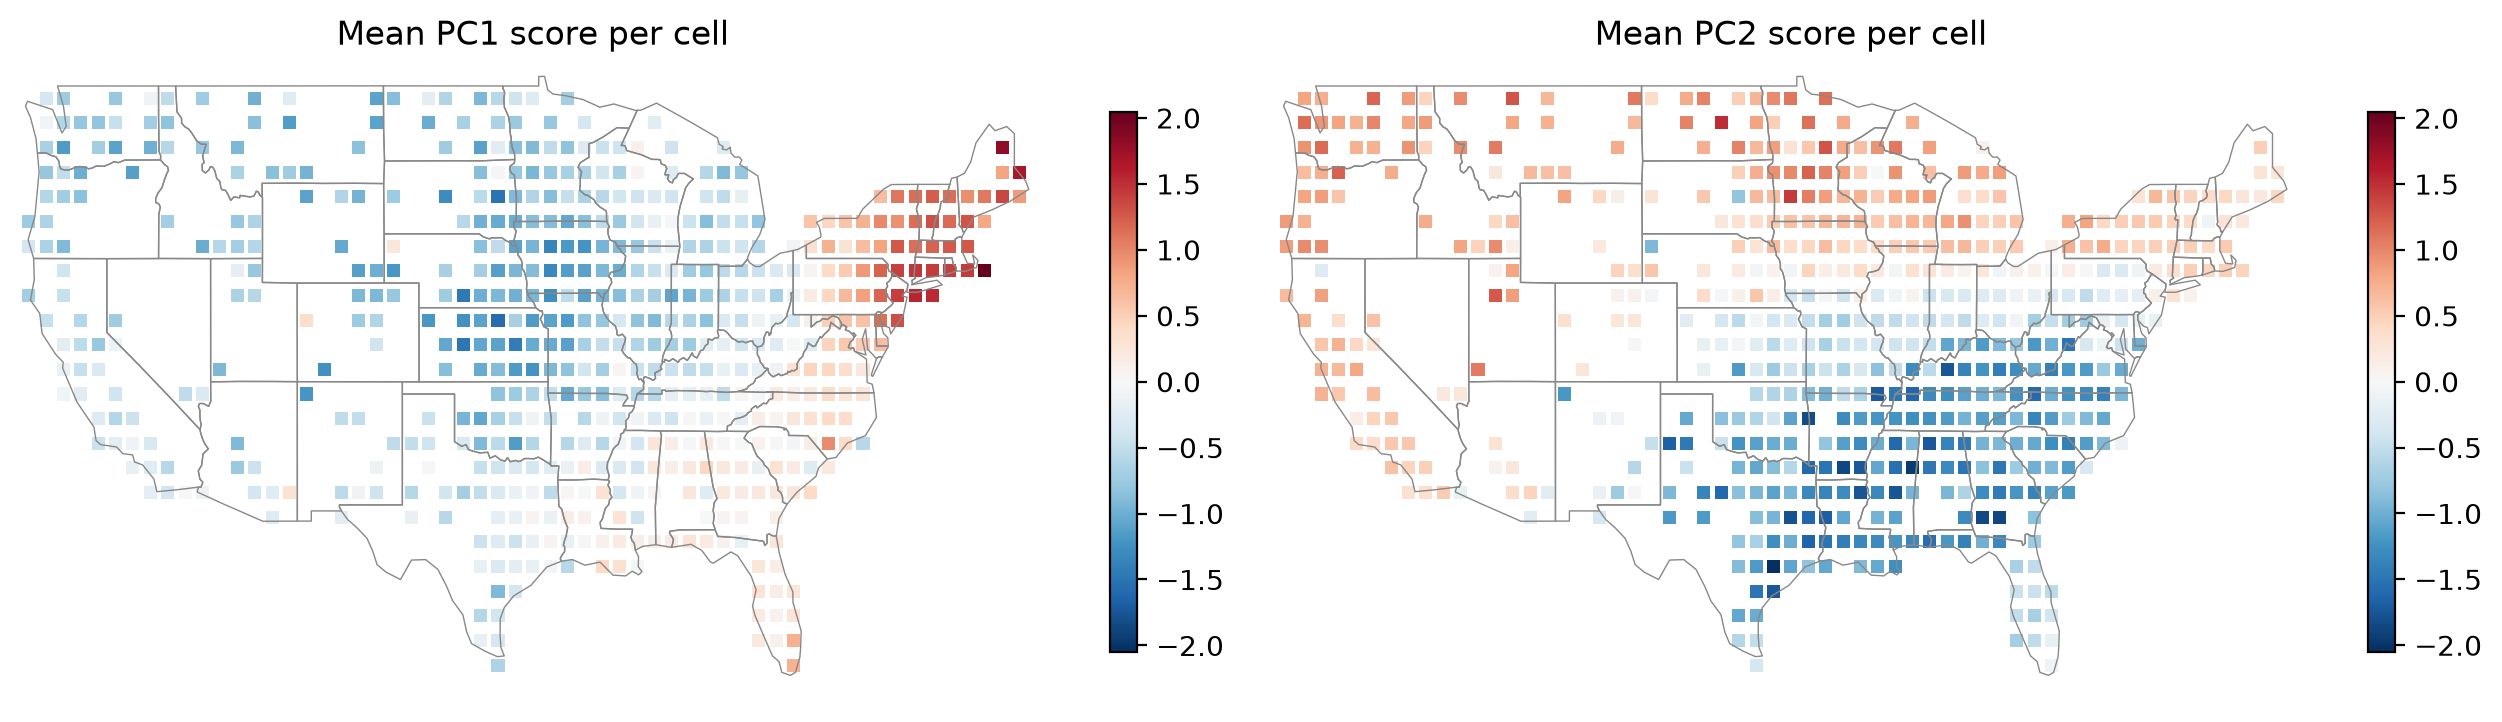
\includegraphics[width=0.95\textwidth]{figures/pca_maps.png}
\caption{Mean PC1 (left) and PC2 (right) score in each $1^\circ \times 1^\circ$ cell with at least 5 respondents (centering only).}
\label{fig:pca_maps}
\end{figure}

\subsection{t-SNE}

PCA can only find straight-line directions, so I also tried t-SNE, which tries to keep each respondent close to their most similar respondents in a 2-D picture. Because t-SNE is slow, it was run on a random sample of 10{,}000 respondents, after first reducing the centered data to its top 50 principal components, with perplexity 50 (only this setting was tried). Figure~\ref{fig:tsne} is consistent with PCA: western respondents form one dense region, eastern respondents another, and southern (low latitude) respondents a third at the bottom, with the groups blending into each other rather than separating cleanly. t-SNE distances within a neighborhood are meaningful, but distances between far-apart regions and the size of each region are not, so the picture should not be used to count groups.

\begin{figure}[h]
\centering
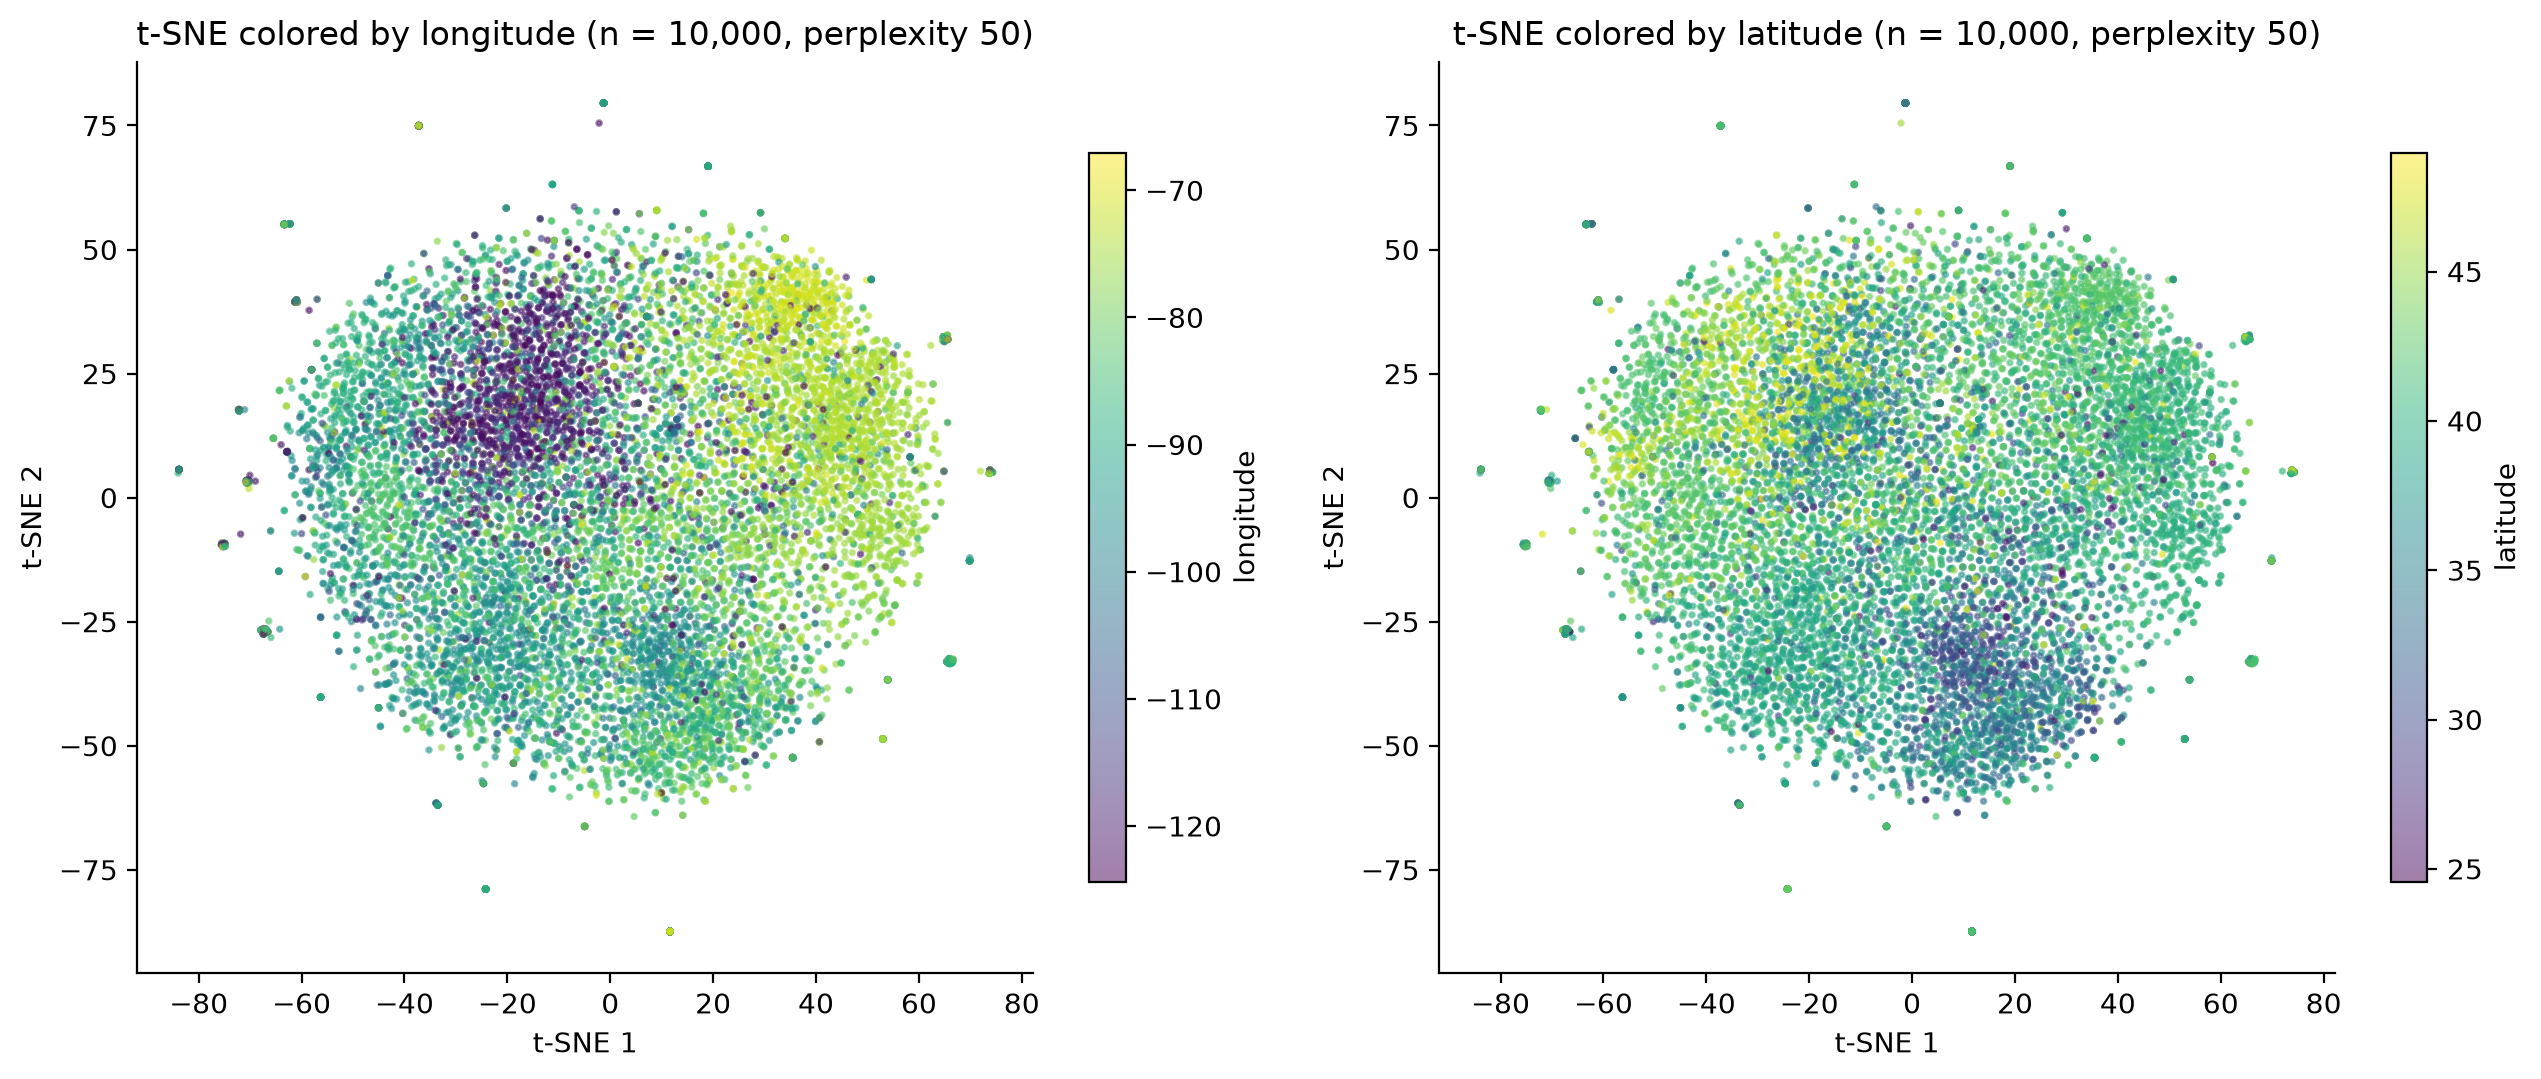
\includegraphics[width=0.9\textwidth]{figures/tsne.png}
\caption{t-SNE of 10{,}000 randomly sampled respondents, colored by longitude (left) and latitude (right).}
\label{fig:tsne}
\end{figure}

\paragraph{Broader takeaways.} Both methods show that dialect answers have a real geographic structure, mostly a Northeast--rest axis and a South--rest axis, but that it is gradual and accounts for a small part of the total variation between people.

\section{Clustering}\label{clustering}

The respondents (rows) were clustered, each described by their scores on the first 20 principal components of the centered one-hot data from Section~\ref{dimension-reduction}. Using 20 components instead of all 468 columns is faster and removes low-variance noise, at the cost of some detail. Two methods were used: k-means, which assigns every respondent to exactly one cluster and assumes roughly round clusters of similar size, and a Gaussian mixture model (GMM) with diagonal covariance, which allows clusters of different sizes and gives each respondent a probability of belonging to each cluster.

\subsection{Choosing the number of clusters}

Figure~\ref{fig:choose_k} shows three measures for 2 to 10 clusters. The k-means inertia decreases steadily with no elbow, and the BIC of the GMM falls sharply from 3 to 4 clusters and then keeps decreasing slowly, so neither points to a clear number. The silhouette score, which compares how close a respondent is to its own cluster versus the nearest other cluster, is highest at $K = 3$ (0.093) but is low for every $K$ (0.070 to 0.093), meaning no choice of $K$ gives well-separated clusters. I used $K = 3$ because it has the highest silhouette, because k-means and the GMM agree closely at this value, and because it gives groups that are easy to interpret. This is a judgment call, and the BIC suggests that more clusters would fit the data better.

\begin{figure}[h]
\centering
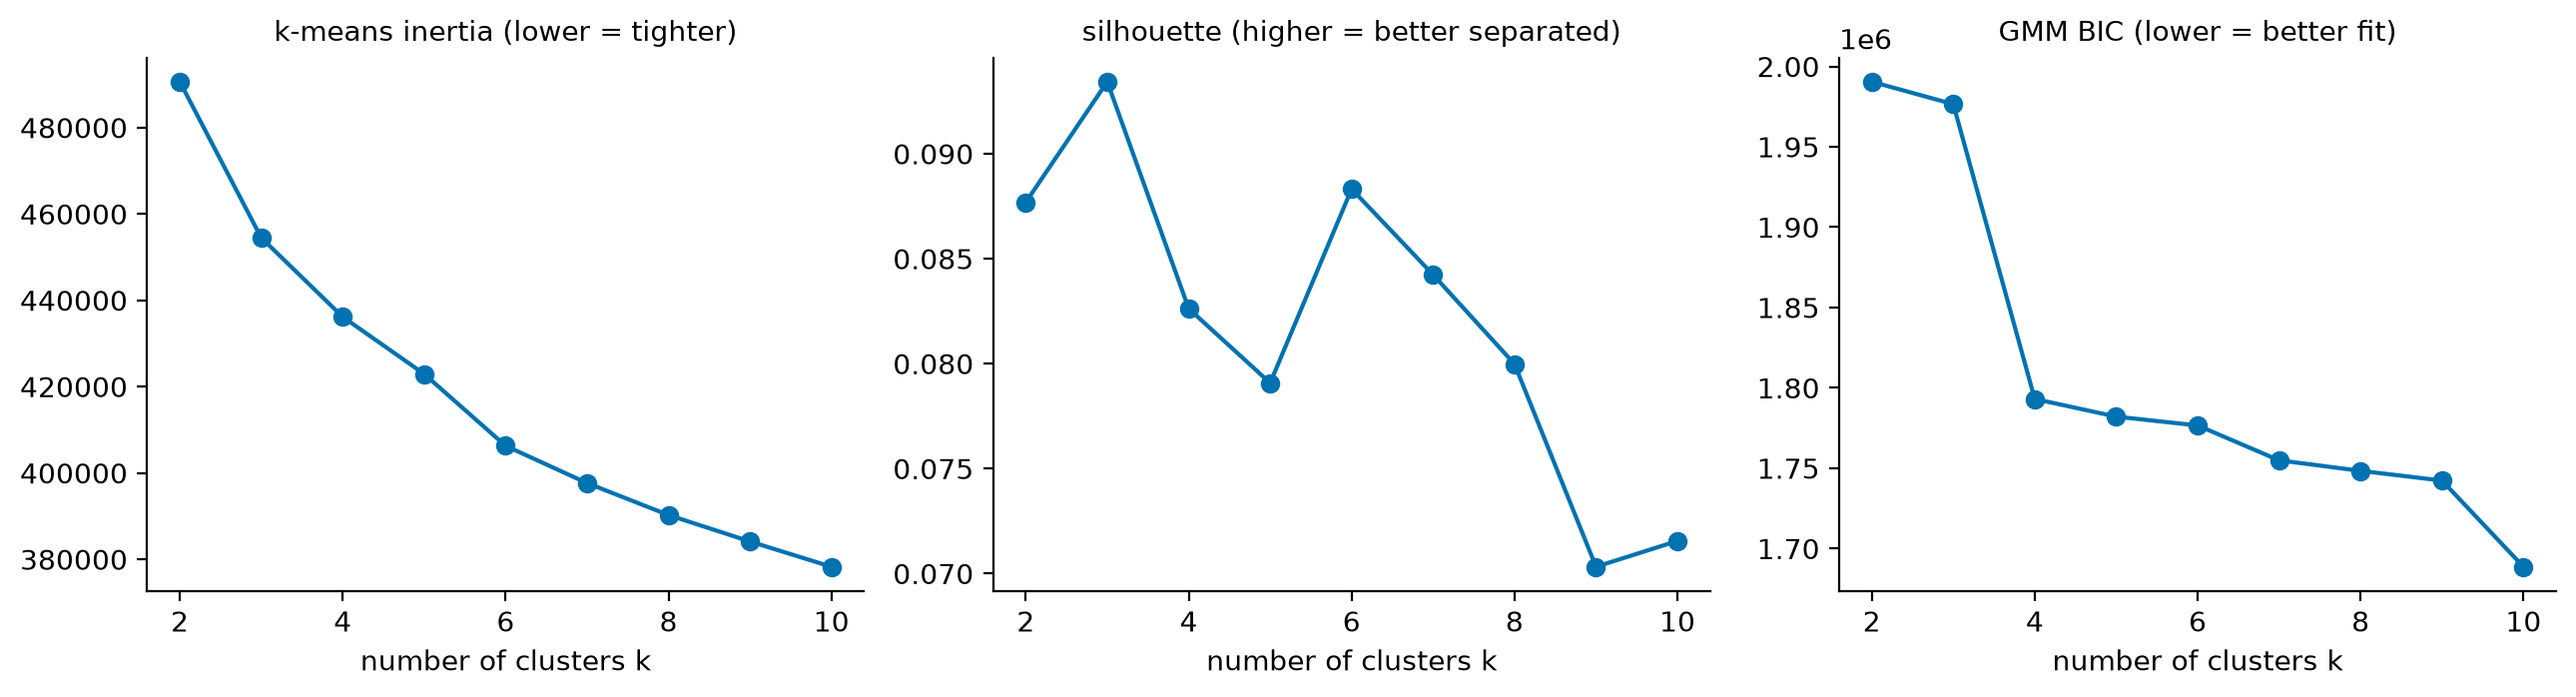
\includegraphics[width=0.95\textwidth]{figures/cluster_choose_k.png}
\caption{Choosing the number of clusters $K$: k-means inertia (left), silhouette score (middle) and GMM BIC (right).}
\label{fig:choose_k}
\end{figure}

\subsection{Results for $K = 3$}

The k-means clusters have 13{,}098, 19{,}100 and 12{,}797 respondents, and the GMM clusters have 11{,}445, 19{,}847 and 13{,}703. The two methods agree closely (adjusted Rand index 0.81, where 1 means identical groupings), so the result does not depend much on the method. Figure~\ref{fig:cluster_maps} maps the most common cluster in each $1^\circ \times 1^\circ$ cell. The three clusters are geographic: one covers the Northeast (blue), one the North and West (orange), and one the South (green). The clusters were found from the answers only, and location was not used, so this agreement with geography is a result of the analysis.

\begin{figure}[h]
\centering
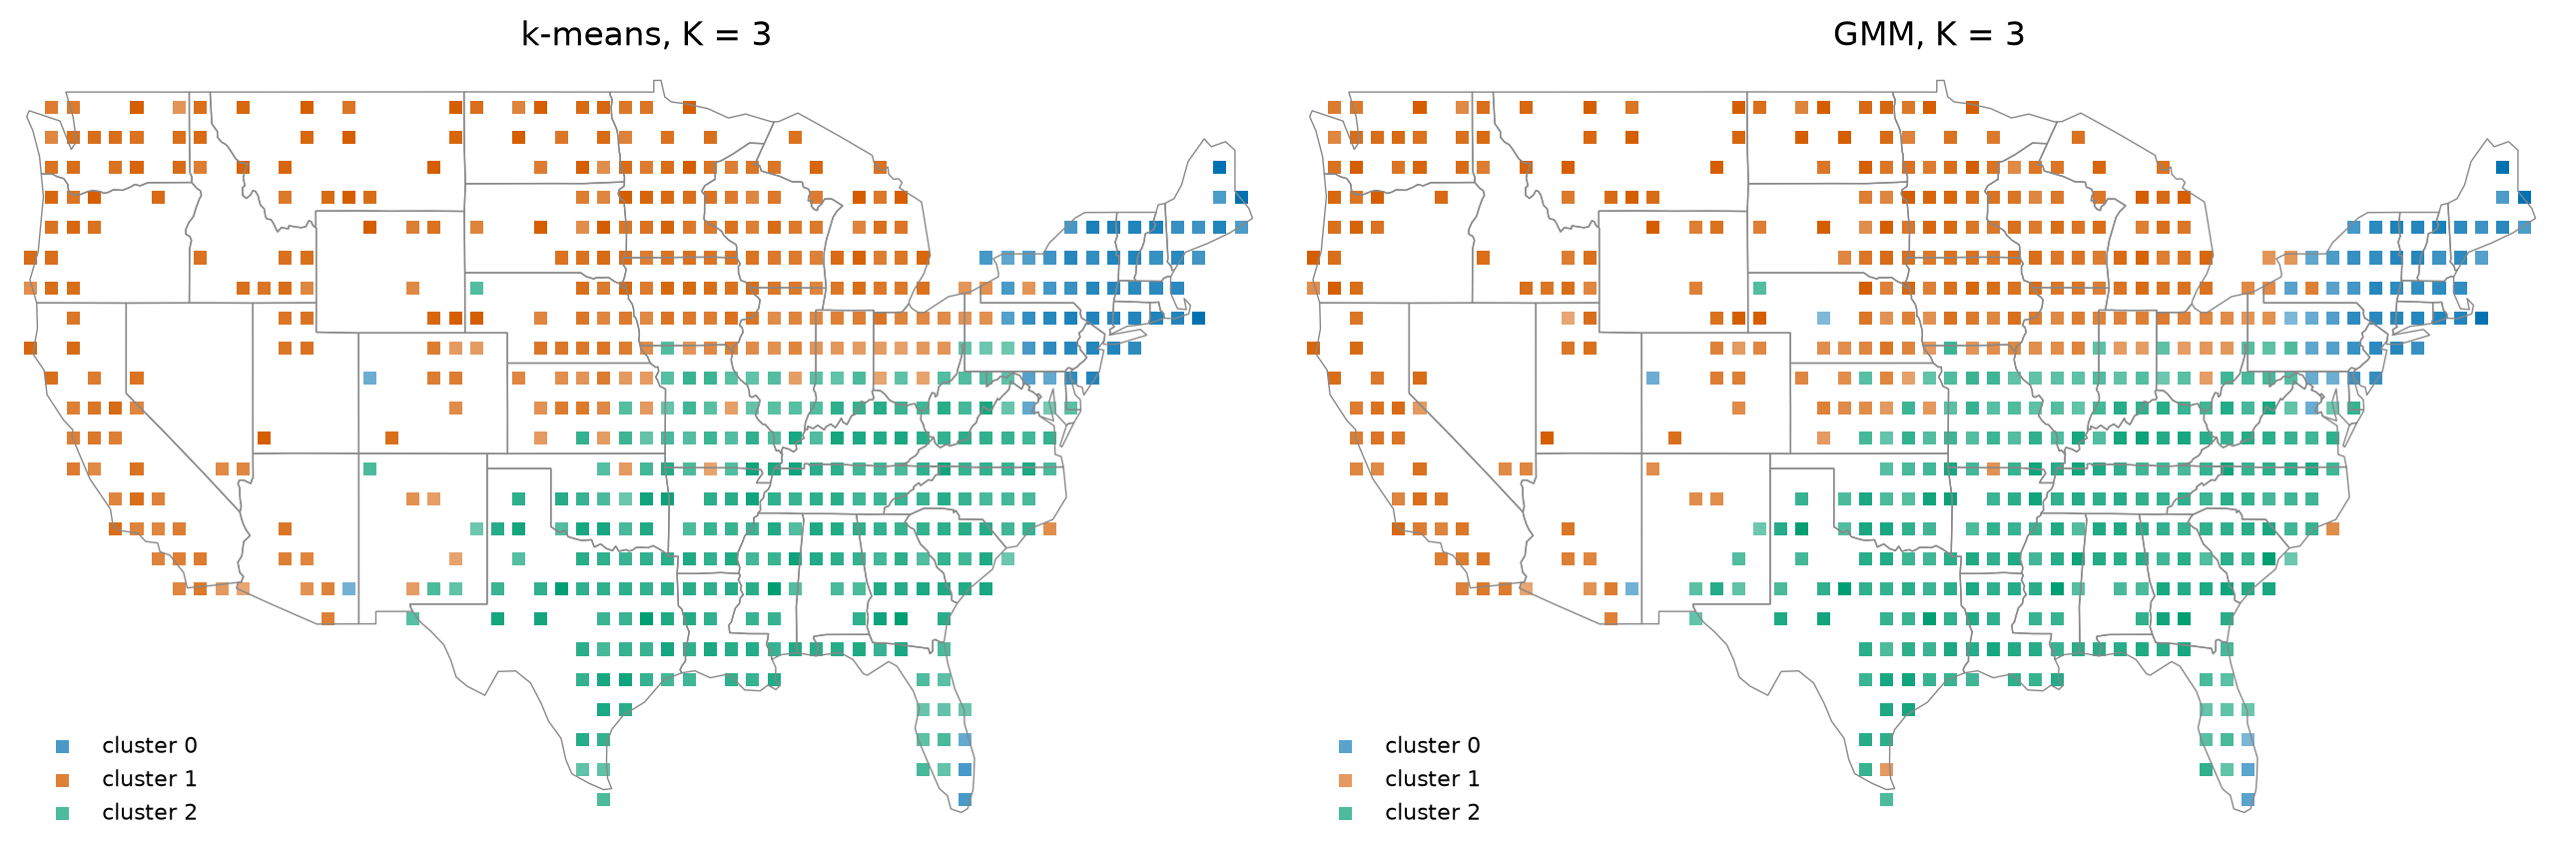
\includegraphics[width=\textwidth]{figures/cluster_maps.png}
\caption{Most common cluster in each $1^\circ \times 1^\circ$ cell (cells with at least 5 respondents) for k-means (left) and the GMM (right). Lighter squares are cells where the cluster is less dominant.}
\label{fig:cluster_maps}
\end{figure}

To see what separates the clusters, Cram\'er's $V$ was computed between the k-means cluster and each question. The strongest are Q105 (soda, pop or coke) and Q073 (sneakers or tennis shoes), each with $V = 0.49$, followed by Q076 (kitty-corner or catty-corner), Q106, Q050 (y'all) and Q103 (water or drinking fountain). Table~\ref{tab:clusters} lists the answers most over-represented in each cluster. The cluster names are my reading of the map and these answers, not something the algorithm produced.

\begin{table}[h]
\centering
\small
\begin{tabular}{llr}
\hline
Cluster (size) & Answer & Share in cluster vs overall \\
\hline
Northeast (13,098) & ``sneakers'' (Q073) & 89\% vs 38\% \\
 & ``soda'' (Q105) & 84\% vs 47\% \\
 & ``sunshower'' (Q080) & 61\% vs 31\% \\
North and West (19,100) & ``kitty-corner'' (Q076) & 75\% vs 47\% \\
 & ``drinking fountain'' (Q103) & 64\% vs 34\% \\
 & ``pop'' (Q105) & 52\% vs 29\% \\
South (12,797) & ``catty-corner'' (Q076) & 70\% vs 34\% \\
 & ``y'all'' (Q050) & 49\% vs 18\% \\
 & ``coke'' (Q105) & 40\% vs 14\% \\
\hline
\end{tabular}
\caption{Answers most over-represented in each k-means cluster (percent of respondents in the cluster who gave the answer, compared with all respondents).}
\label{tab:clusters}
\end{table}

\subsection{Separate groups or a continuum?}

Figure~\ref{fig:continuum} (left) shows the respondents in the PC1--PC2 plane, colored by cluster. The clusters touch and overlap rather than forming separated clouds, and the cluster boundaries are straight cuts through one connected cloud. The GMM probabilities (right) agree: most respondents are assigned with high confidence, but 23\% have a probability below 0.8 for their most likely cluster. Together with the low silhouette scores, this suggests that the three clusters are best read as regions along a gradient of dialect, not as three separate groups of speakers.

\begin{figure}[h]
\centering
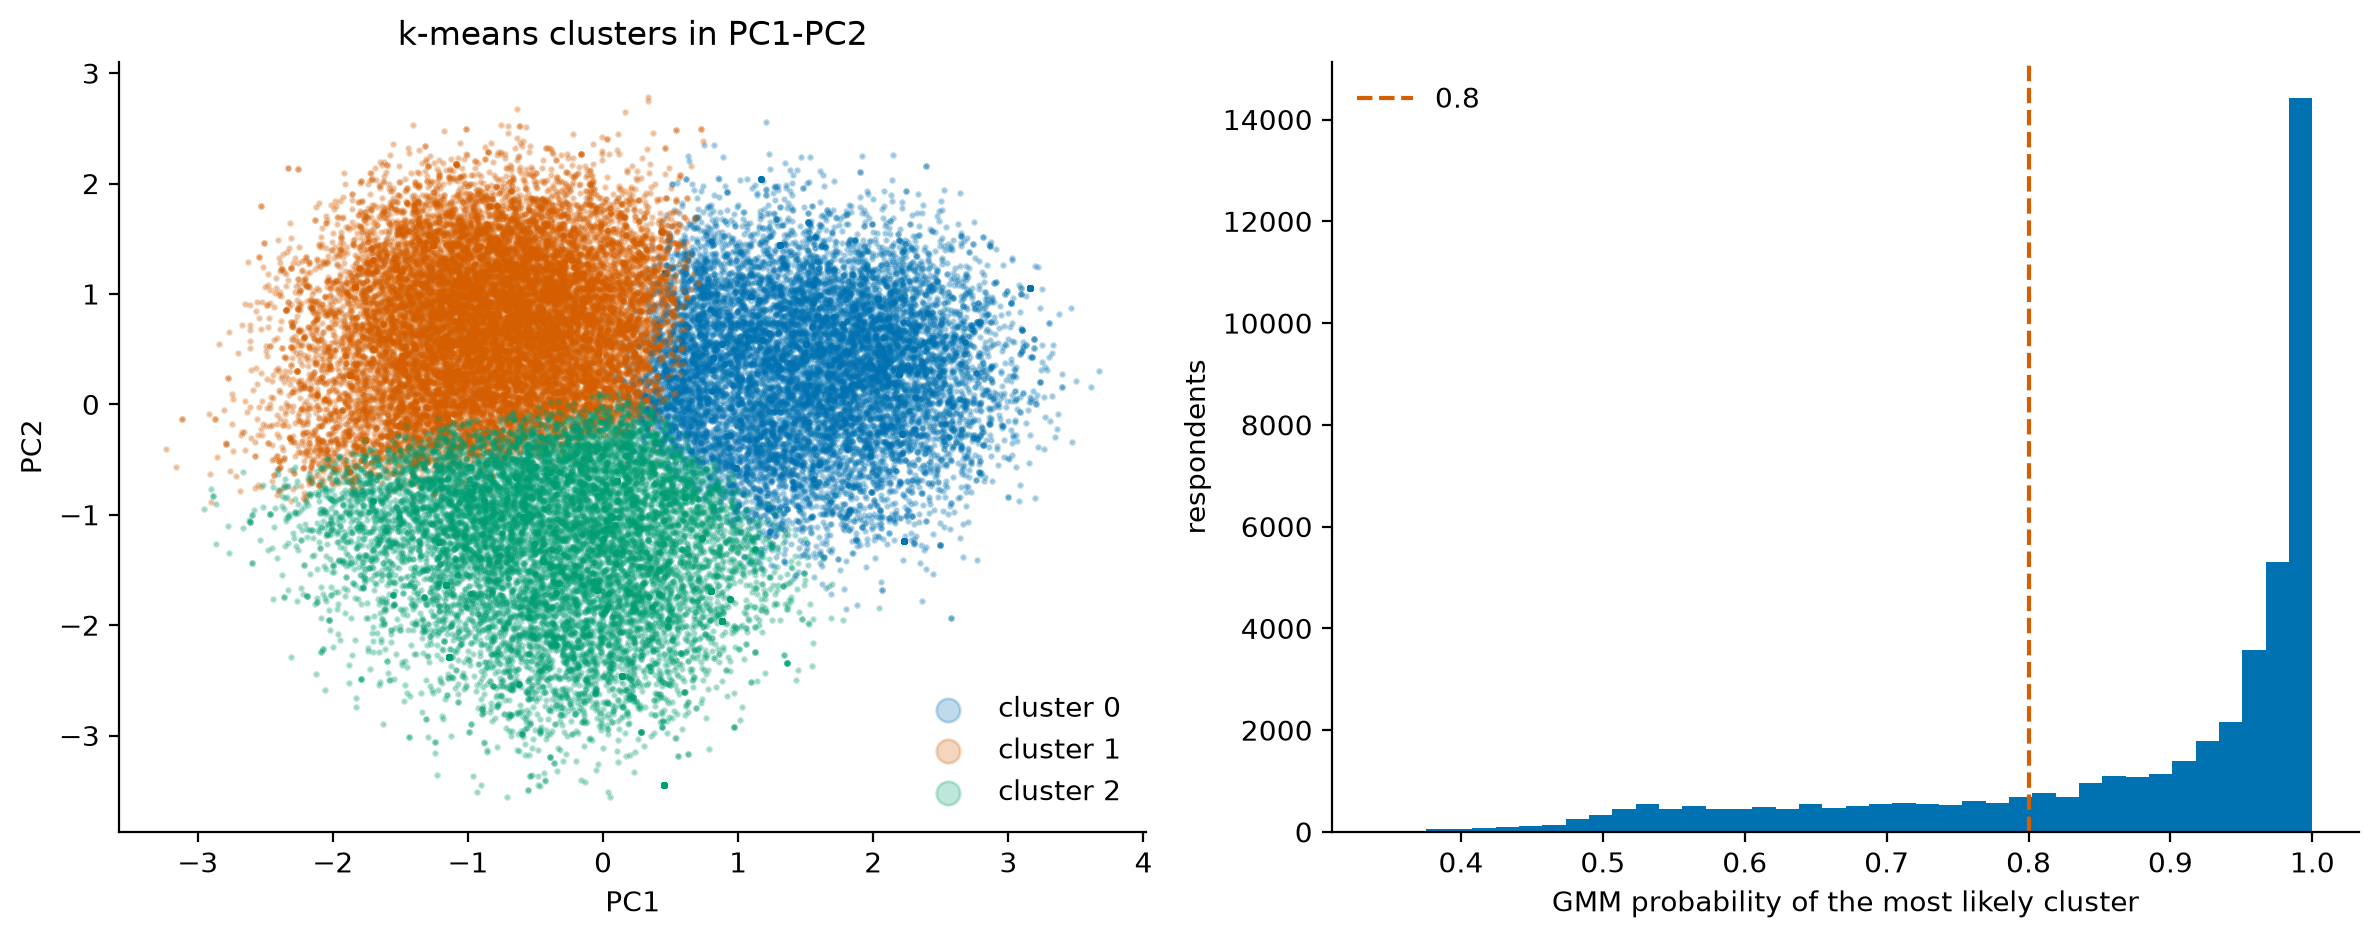
\includegraphics[width=0.9\textwidth]{figures/cluster_continuum.png}
\caption{Left: respondents in PC1--PC2 colored by k-means cluster. Right: for each respondent, the GMM probability of the most likely cluster (the dashed line is 0.8).}
\label{fig:continuum}
\end{figure}

\section{Stability of Findings to Perturbation}\label{stability}

I tested how stable the three k-means clusters from Section~\ref{clustering} are in two ways, and measured agreement with the original clustering using the adjusted Rand index (ARI): 1 means identical groupings, about 0 means no better than chance, and the cluster numbering does not matter. Only the $K = 3$ k-means clustering was tested.

\paragraph{Different starting points.} k-means can end at different solutions depending on where it starts. I re-ran k-means 30 times on the same data, each from a single random initialization, and compared each result with the original clustering (the best of 20 starts). The ARI was between 0.94 and 1.00 for every run (median 0.95), so the starting point changes the result very little (Figure~\ref{fig:stability}, left).

\paragraph{Perturbing the data.} I then drew 30 bootstrap samples of the respondents (sampling with replacement, the same size as the data). For each sample the whole procedure was repeated: PCA was refit, k-means was run on the resampled respondents, and every original respondent was assigned to the nearest new cluster. The ARI against the original clustering was between 0.92 and 0.99 (median 0.98; Figure~\ref{fig:stability}, middle). To check each cluster separately, I matched every original cluster with its best-matching new cluster and computed the Jaccard similarity (overlap divided by combined size). The average was 0.98 for all three clusters, well above the usual rule of thumb of 0.75 for a stable cluster (Figure~\ref{fig:stability}, right). Overall, 96.5\% of respondents were placed in their original cluster in at least 90\% of the bootstraps. Figure~\ref{fig:stability_map} shows that this share is close to 1 in almost every cell, and the cells with lower values lie mostly where the clusters meet, such as parts of the Plains and Midwest.

\begin{figure}[h]
\centering
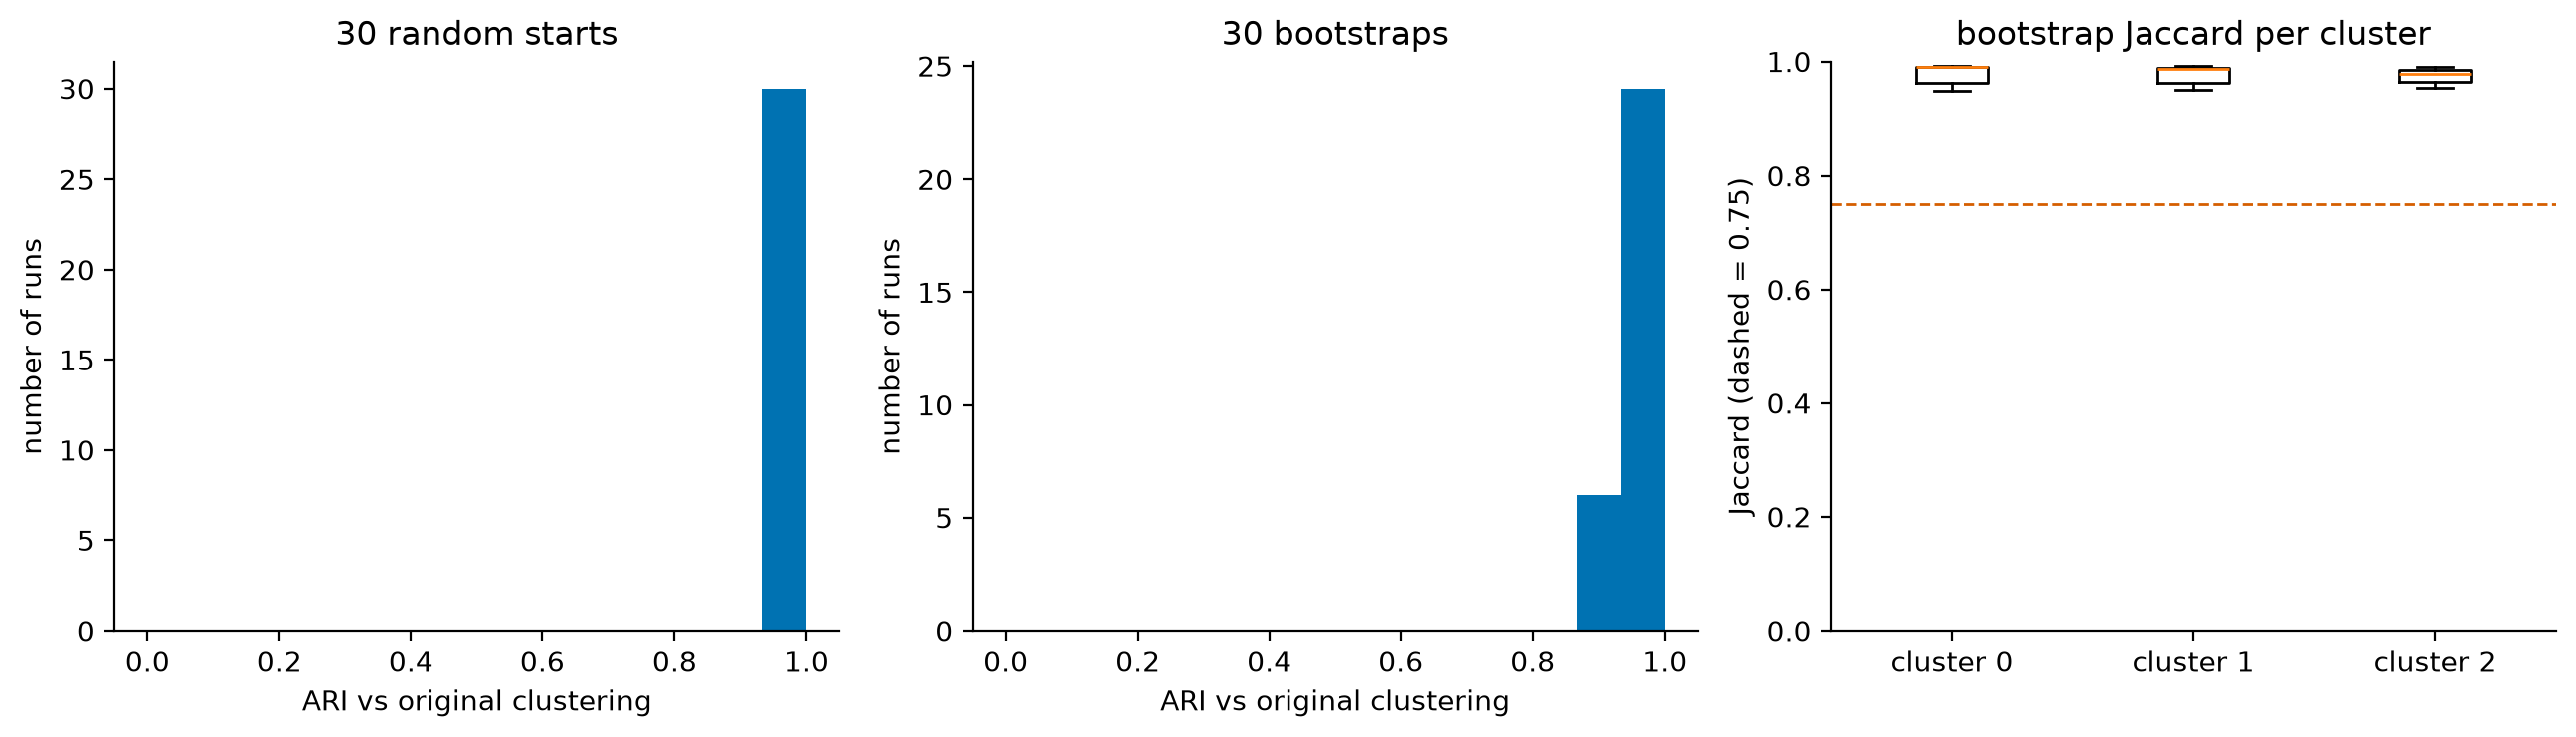
\includegraphics[width=0.95\textwidth]{figures/stability.png}
\caption{Left: ARI between the original clustering and 30 k-means runs with random starting points. Middle: ARI between the original clustering and 30 bootstrap re-clusterings. Right: bootstrap Jaccard similarity for each cluster (the dashed line is 0.75).}
\label{fig:stability}
\end{figure}

\begin{figure}[h]
\centering
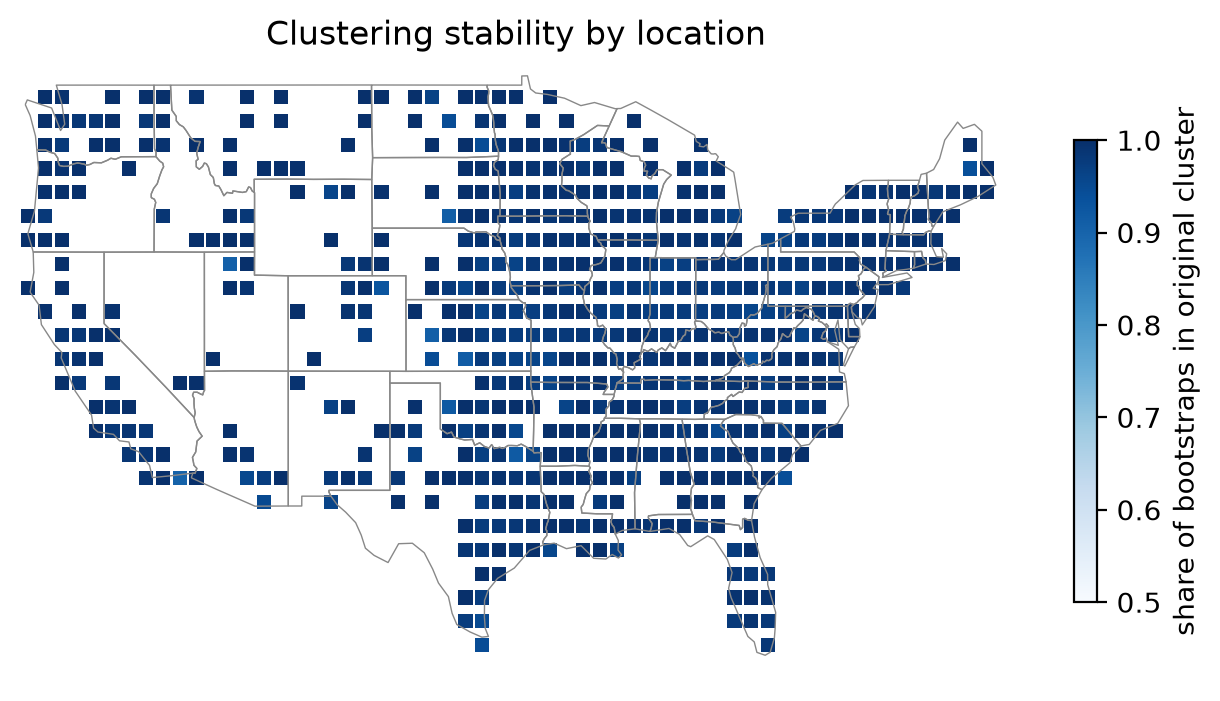
\includegraphics[width=0.55\textwidth]{figures/stability_map.png}
\caption{For each $1^\circ \times 1^\circ$ cell (at least 5 respondents), the average share of bootstraps in which respondents were assigned to their original cluster.}
\label{fig:stability_map}
\end{figure}

\paragraph{Overall stability findings.} The clustering is stable: different starting points and resampled data give nearly the same three groups. This does not show that the three groups are real, separate dialect communities. k-means will split any cloud of points into a fixed number of regions, and a smooth gradient can be cut in a similar place every time. Combined with the low silhouette scores and the overlapping clusters in Section~\ref{clustering}, the conclusion is that the three regions are a stable summary of a continuum.

\section{Conclusion}\label{conclusion}

\subsection{Main takeaways}

Dialect answers in this survey have a real geographic structure. The first two principal components are a Northeast-versus-rest axis and a South-versus-rest axis, and k-means and a Gaussian mixture model both split the respondents into three groups (Northeast, North and West, South) without using location. The main questions behind these groups are the generic term for a soft drink (Q105), the term for gym shoes (Q073), and the terms for the corner across the street (Q076) and for a group of people (Q050). The groups are stable under different starting points and bootstrap resamples (ARI at least 0.92). However, the regional signal explains only a small share of the variation between people (the first 20 principal components explain 33\%), the silhouette scores are low, and the clusters touch and overlap. I conclude that the three groups are a stable summary of a smooth gradient across the country, not three separate dialect communities.

\subsection{The three realms of data science}

 The data are useful for describing how word choice varied across the US at the time of the survey, but I would be careful using them for future decisions. Respondents were self-selected online volunteers, so they are not representative of the population, and the survey is no longer running, so the answers are a snapshot that may not match current usage. The location is a latitude and longitude assigned from the reported city and state, and it is where a person lives, not necessarily where they grew up, which blurs the link between a person's answers and a place. Finally, skipped answers occur only for respondents with ID up to about 17{,}000, so missingness is not uniform across the sample.  Several choices could change the results: how skipped answers are handled (I left them as all zeros after one-hot encoding), centering without scaling, using 20 principal components, and choosing $K = 3$ with weak support from the silhouette score and BIC. The stability analysis shows that the clustering is stable to resampling and starting points, but only for $K = 3$ and k-means, and a stable clustering is not the same as a correct one. The clusters could be used to place a new respondent by assigning them to the nearest cluster, and the stability results suggest that this would be consistent for respondents like those in the survey. I would trust it less for a different population (for example, younger respondents or a different sampling method), because the clusters describe this particular sample. The clusters are suited to broad regional summaries, such as which of the three groups a region resembles, and not to deciding anything about an individual, since 23\% of respondents have a probability below 0.8 for their most likely cluster.

\subsection{A reality check}

A clustering is only useful if it matches something outside the algorithm. I would compare the cluster map with published dialect-region maps from the dialectology literature. If the clusters are real, their boundaries should be close to the boundaries linguists have identified, and I would measure this by the share of respondents whose cluster agrees with the region of their location. I would also leave out one question (for example, Q105), repeat the PCA and clustering using the other 66 questions, and check whether the clusters still differ in their answers to the held-out question, compared with clusters formed from random groups of the same sizes. This tests whether the clusters capture dialect in general and not only the particular questions used to form them. Also, cluster a random half of the respondents, assign the other half to the nearest cluster, and see whether their assignments agree with clustering that half directly.

\section{Academic Honesty}\label{academic-integrity-statement}
 
\subsection{Statement}
 
Dear Bin,
I affirm that the work in this report is my own, and that all sources I used, including any discussions with
classmates, are properly cited. Academic research honesty is necessary as it is the foundation of trust in
science and the integrity of the field at large. Not only do we as researchers have an obligation to be honest
to ourselves, our labs, and the greater scientific community when it comes to research, but also to the public,
as many of us are funded by tax dollars and want our findings to be helpful to humanity.
 
\subsection{LLM Usage}
Claude was used for debugging issues and slight refinement of text.  
\subsection{Collaborators}
 
N/A 

 
\begin{thebibliography}{9}
\small
\bibitem{nk2003} Nerbonne, J. and Kretzschmar, W. (2003). Introducing computational techniques in dialectometry. \emph{Computers and the Humanities}, 37(3):245--255.
\bibitem{nk2006} Nerbonne, J. and Kretzschmar, W. (2006). Progress in dialectometry: toward explanation. \emph{Literary and Linguistic Computing}, 21(4):387--397.
\bibitem{vaux} Vaux, B. Dialect Survey. \url{https://www.dialectsofenglish.com/} (the questions and answers were obtained from \url{http://dialect.redlog.net/index.html}).
\end{thebibliography}
 
\end{document}